\subsection{
  Replies to comments received from Nakadaira-san - Jan. 14, 2013 }

\begin{enumerate}

%........................................................................................................
\vspace{5 mm}
\item
{\em
  ``P.28, l.626~628 : "although it is ... to have pathological behaviour."
  I can not understand at all for this statement, because the apparent
  oscillation amplitude can be greater than 1 because of the statistical
  error, the too conservative assumption on the energy resolution, etc.
  I think that the limiting at $sin^2(2\theta_{23})<=1$ make the non-Gaussian
  behaviour of the pull distributions large.
  I think that you can draw the contour plot within the physical region
  even you use the fitter without limiting because you are adopting the
  Feldman-Cousin method.''
}\\
\\
The oscillation probability is a function of $E_{true}$, not $E_{reco}$.
Therefore, in order to apply oscillations, the functional dependence of the p.d.f. on $E_{true}$
needs to be known.
This analysis uses a 2-dimensional p.d.f. defined in ($E_{reco}$, $E_{true}$) space,
as mentioned in various places in the text.
Values of $\sin^2(2\theta_{23})>1$, cause the contents of some of the 2-dimensional p.d.f
bins to become negative, which is clearly pathological (meaningless) 
as the content of each bin represents a probability. 

In addition, we do not interpret the results in a simple 2-flavour framework where
the oscillation amplitude can be seen as an effective one,
and where values greater than 1 can be somewhat understood.
In our 3-flavour oscillation framework, values of $sin^2(2\theta_{23})>1$ are, again,
meaningless.

We think that the last statement ({\em ``you can draw the contour plot within the physical region
even you use the fitter without limiting because you are adopting the
Feldman-Cousins method.''}) is incorrect. The Feldman-Cousins prescription 
clearly states that the best fit is ``for the physically allowed values of 
$\sin^2(2\theta_{23})$ and $\Delta m^{2}$'' (Phys. Rev. D 57, 3873, section 
V B).

%........................................................................................................
\vspace{5 mm}
\item
{\em
  ``P.29 l.660~663 : "D.Karlen has ... samples” 
  I read the Dean's presentation, and I totally agree with him. I think
  that it is possible to estimate the $\chi^2$ for shape using the usual
  definition, (N\_obs-N\_exp)$^2$/(Error of N\_exp)$^2$, because you have
  estimated the errors of each bin in Fig.18.
  But I think that its priority is not urgent. I do not think it is not
  so important to check the goodness-of-fit of ML fit with $\chi^2$.
  I think that the key of Dean's suggestion is that the likelihood ratio
  is not good approximation of the $\chi^2$ for the statistics of the nu\_mu
  disappearance analysis. So, The statement in L.639~642, P.29 ("The
  advantage of the likelihood ... interchangeably.") is not applicable
  for this tech note.''
}\\
\\
We also agree with Dean. The goodness-of-fit test implemented in this analysis
is the one suggested by Dean, as mentioned in various places in the text.

The statement in L.639~642 is a general comment on the advantage of using the likelihood ratio.
The comment is, in fact, applicable to this analysis if a coarser binning is used
(i.e. as was done in the test suggested by Dean). In Fig.\ \ref{fig:chisq}, 
the distribution of likelihood ratios, for the 5 reconstructed energy bins used in the
goodness-of-fit test, and for the Run 1+2+3 exposure is shown.
As it can be seen, even with the current statistics, this distribution approaches the
the $\chi^{2}$ distribution with 2 degrees of freedom, also shown on the same plot.

\begin{figure*}[htb]
\center
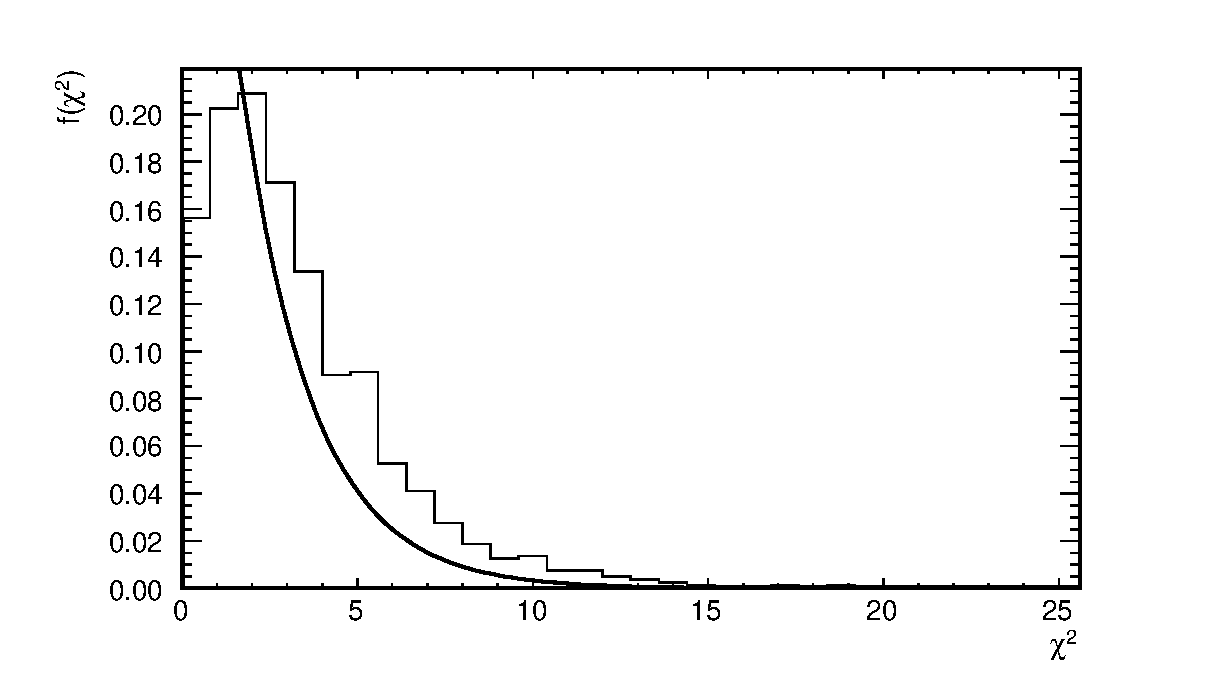
\includegraphics[width=25pc]{./images/ourchisqgof_and_chisq.eps}
\caption {
  Distribution of likelihood ratios, for the 5 reconstructed energy bins used in the
  goodness-of-fit test, and for the Run 1+2+3 exposure.
  This is the same distribution as the one shown in Fig.33 in T2K-TN-141 and further.
  details can be found there-in.
  The continuous distribution, shows the $\chi^2$ distribution with 2 degrees of freedom.
}
\label{fig:chisq}
\end{figure*}

%........................................................................................................
\vspace{5 mm}
\item
{\em
  ``Sec. 4.3, Appendix. H.
  The plot of the pull distributions are described, but it is difficult
  to estimate the fitter bias numerically. Could you add the plots of
  the residuals: (Best fit - input) and the add the estimation of the
  bias, (for example, mean/median/mode of the residual distribution.)  
  We should check the fitter bias is enough smaller than the size of the
  68\% allowed region (the final result of the contour plot.). If the
  fitter bias is not enough small, the best fit point may not be the
  special value within the allowed region. It is quite important when we
  think how to describe the best fit point.
  And It is difficult to understand the meaning of the Fig. 386,
  Fig. 391. Sereral pull distributions are not the normal distribution.
  What does it mean?  Is it OK?
  For example, the 2D plots, the residual(or pull) of $sin^2(2\theta_{23})$
  vs the residual(or pull) of the systematic parameter, may be useful to
  check if the treatment of the certain systematic parameter cause the
  bias of $sin^2(2\theta_{23})$.''
}\\
\\
In version 2 of T2K-TN-141, residual plots were added in Appendix H
and the mean of the distributions is displayed on the statistics box.

The strange shape of certain pull distributions, and in particular of $f_{SF}$,
was addressed in replies to questions sent by other reviewers.
Please see the reply to Anselmo's comment \#9.

At maximal mixing, the mean of the $sin^2(2\theta_{23})$ residual distribution is 0.01.
This is to be compared with a 68\% CL range which is $\sim$ 0.043 (at the best-fit $|\Delta m^2_{32}|$ value).	

A 2-dimensional plot, showing the pull of $sin^2(2\theta_{23})$ vs the
residual of a typical systematic parameter is shown in Fig.\ \ref{fig:nakadaira_q3} in this addendum.
Plots of other systematic parameters look similar.
There is no correlation between the pull of $sin^2(2\theta_{23})$ and the
residuals of the systematic parameters.

\begin{figure*}[htb]
\center
\includegraphics[width=35pc]{{./images/28_all_0.900000_mixpull_skdetccnqeres_rev}.eps}
\caption {
  Pull of $sin^2(2\theta_{23})$ plotted against the residual of systematic parameter $f_{CCnonQE}^{SK}$
  (SuperK CCnonQE efficiency). Plots of other systematic parameters look similar.
  The plot was generated using the `2+8' fit variant, for true oscillation parameters
  $sin^2(2\theta_{23}) = 0.9$ and $|\Delta m^2_{32}| = 2.4 \times 10^{-3} eV^{2}/c^{4}$.
}
\label{fig:nakadaira_q3}
\end{figure*}


%........................................................................................................


\end{enumerate}
